% Project n. 5 na ITY
% Jan Jakub Kubik (xkubik32)
% VUT FIT 15.4.2017


\documentclass{beamer}
\usetheme{Madrid}
\usecolortheme{orchid}


% ---------
% Packages
% ---------
\usepackage[utf8]{inputenc}
\usepackage[czech]{babel}
\usepackage{graphicx}

\usefonttheme{professionalfonts}


% --------------------
% info about document
% --------------------
\title{Internet of things/(IoT)}
\author{Ján Jakub Kubík}
\date{\today}

\begin{document}


% -----------
% Title page
% -----------
\begin{frame}
  \titlepage
\end{frame}


% --------
% Slide 2
% --------
\begin{frame}[t]
  \frametitle{\centerline{Úvod}}
  \begin{center}
    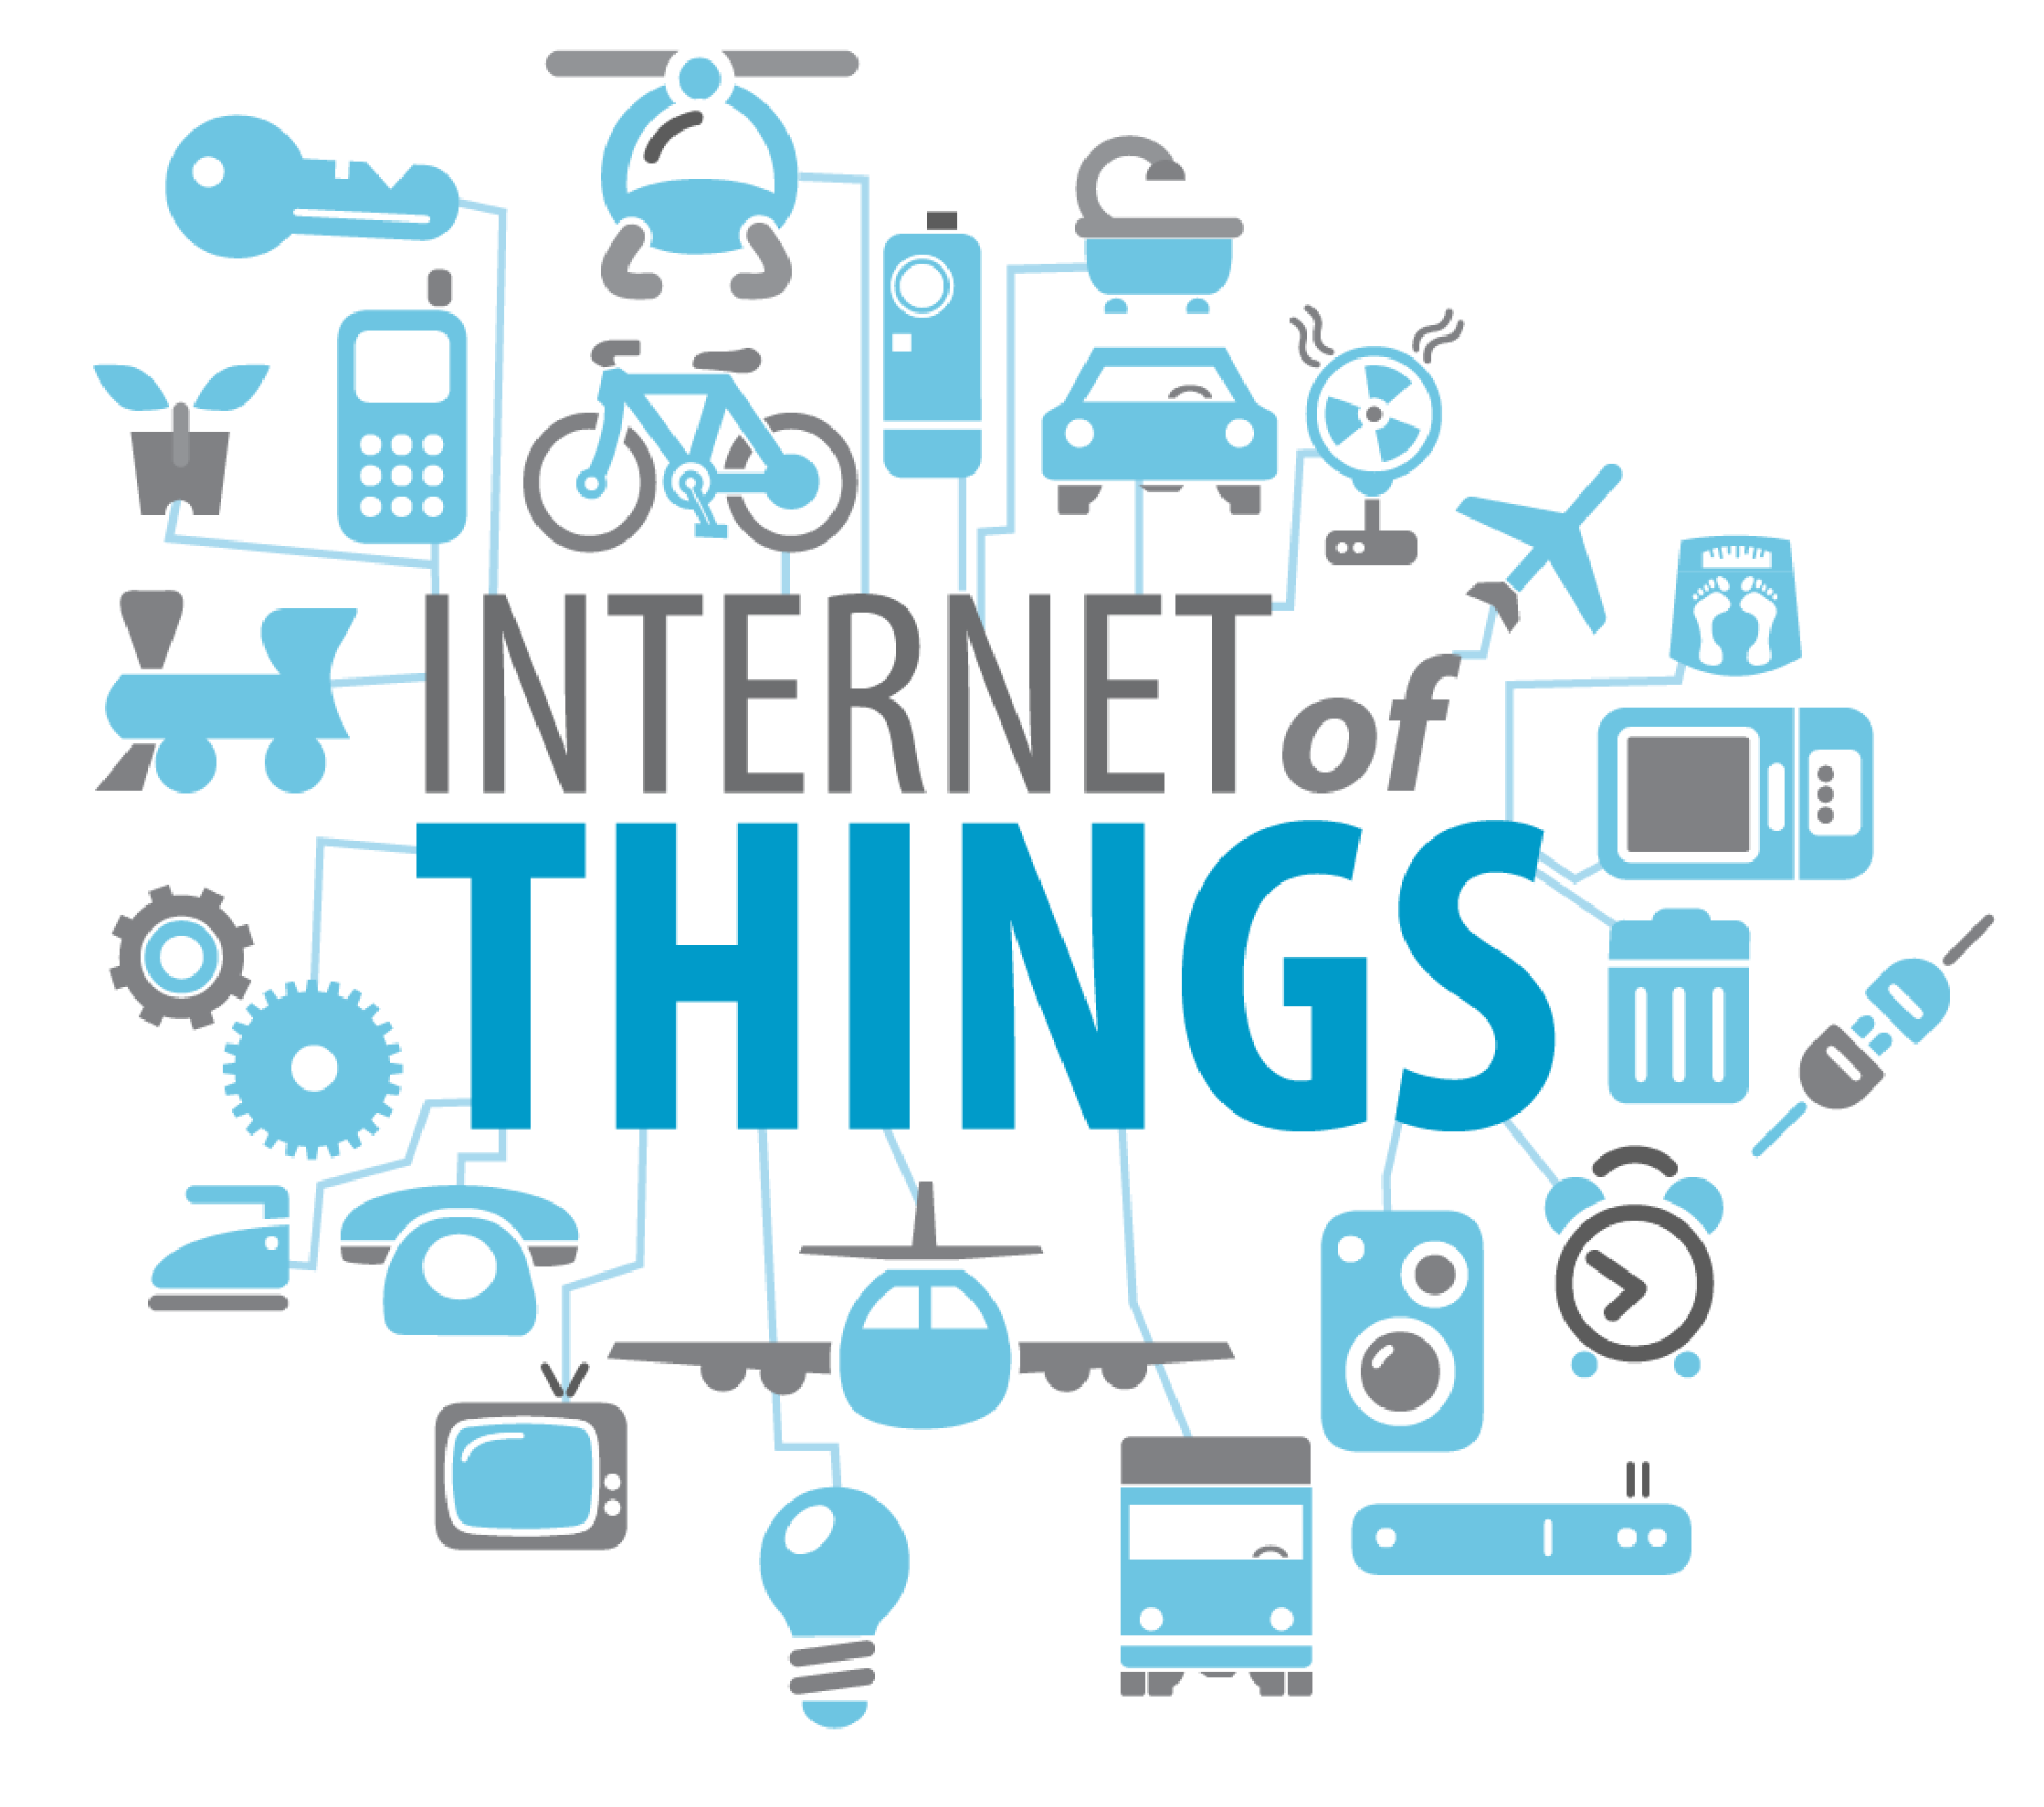
\includegraphics[height=4.5cm]{IoT.eps}
  \end{center}
  \begin{block}{}
    Označenie pre rôzne zariadenia a objekty prepojené pomocou intenetu, ktore sú schopné
    spolu komunikovať vymienať si informácie a reagovať na rôzne podnety
  \end{block}
\end{frame}


% --------
% Slide 3
% --------
\begin{frame}
  \frametitle{\centerline{3 veci na vyriešenie pre úspech IoT}}
  \begin{itemize}
    \item Počítačová gramotnosť
    \item Protokol na komunikáciu
    \item Kapacita pásma pre prenos dat
  \end{itemize}
\end{frame}


% --------
% Slide 4
% --------
\begin{frame}
  \frametitle{\centerline{Vývoj IoT v číslach}}
  \begin{itemize}
    \item Očakáva sa, že do roku 2020 bude spolu prepojených viac ako 50 miliard zariadení
  \end{itemize}
  \begin{center}
    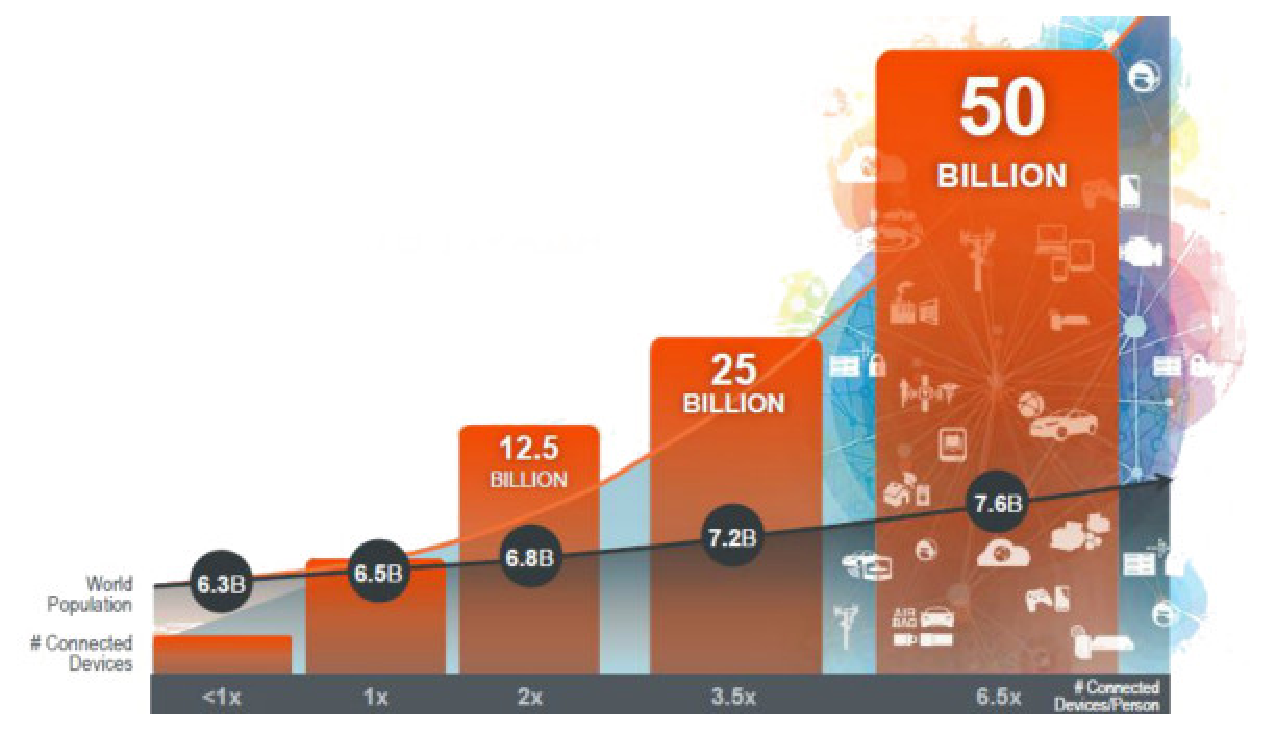
\includegraphics[height=3cm]{Vyvoj_v_cislach.eps}
  \end{center}
\end{frame}


% --------
% Slide 5
% --------
\begin{frame}
  \frametitle{\centerline{Výhody}}
  \begin{columns}[T]
    \begin{column}{.3\textwidth}
      \begin{itemize}
        \item Dáta
        \item Životné prostredie
        \item Úspora času
        \item Úspora peňazí
      \end{itemize}
    \end{column}
    

    % Column 2
    \begin{column}{.5\textwidth}
      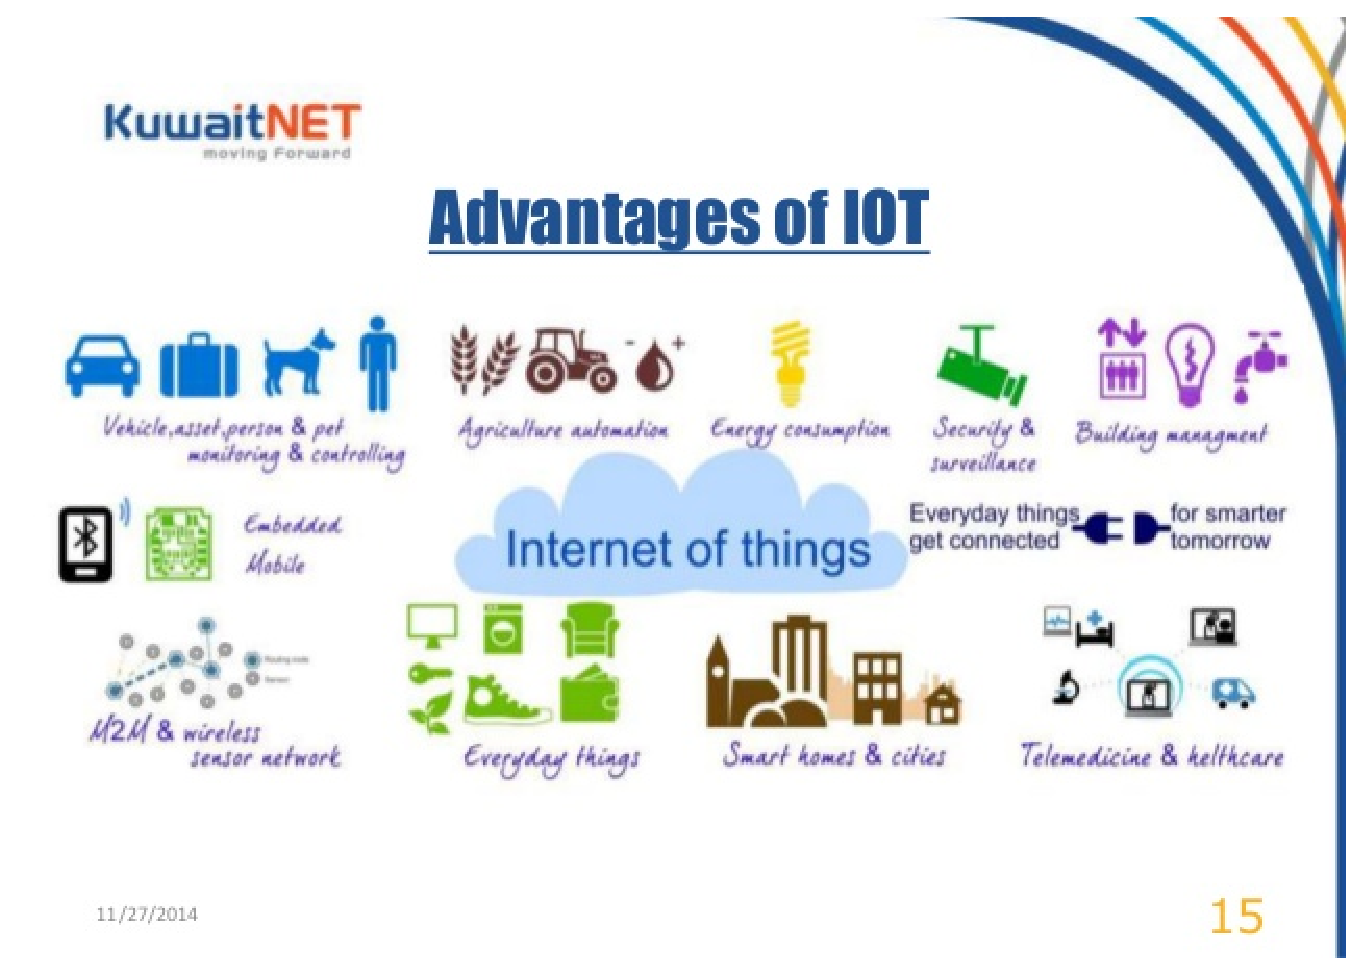
\includegraphics[height=4cm]{IOT_adv.eps}
    \end{column}
  \end{columns}
\end{frame}


% --------
% Slide 6
% --------
\begin{frame}
  \frametitle{\centerline{Nevýhody}}
  \begin{columns}[T]
    \begin{column}{.3\textwidth}
      \begin{itemize}
        \item Komplexnosť
        \item Bezpečnosť
      \end{itemize}
    \end{column}


    % Column 2
    \begin{column}{.5\textwidth}
      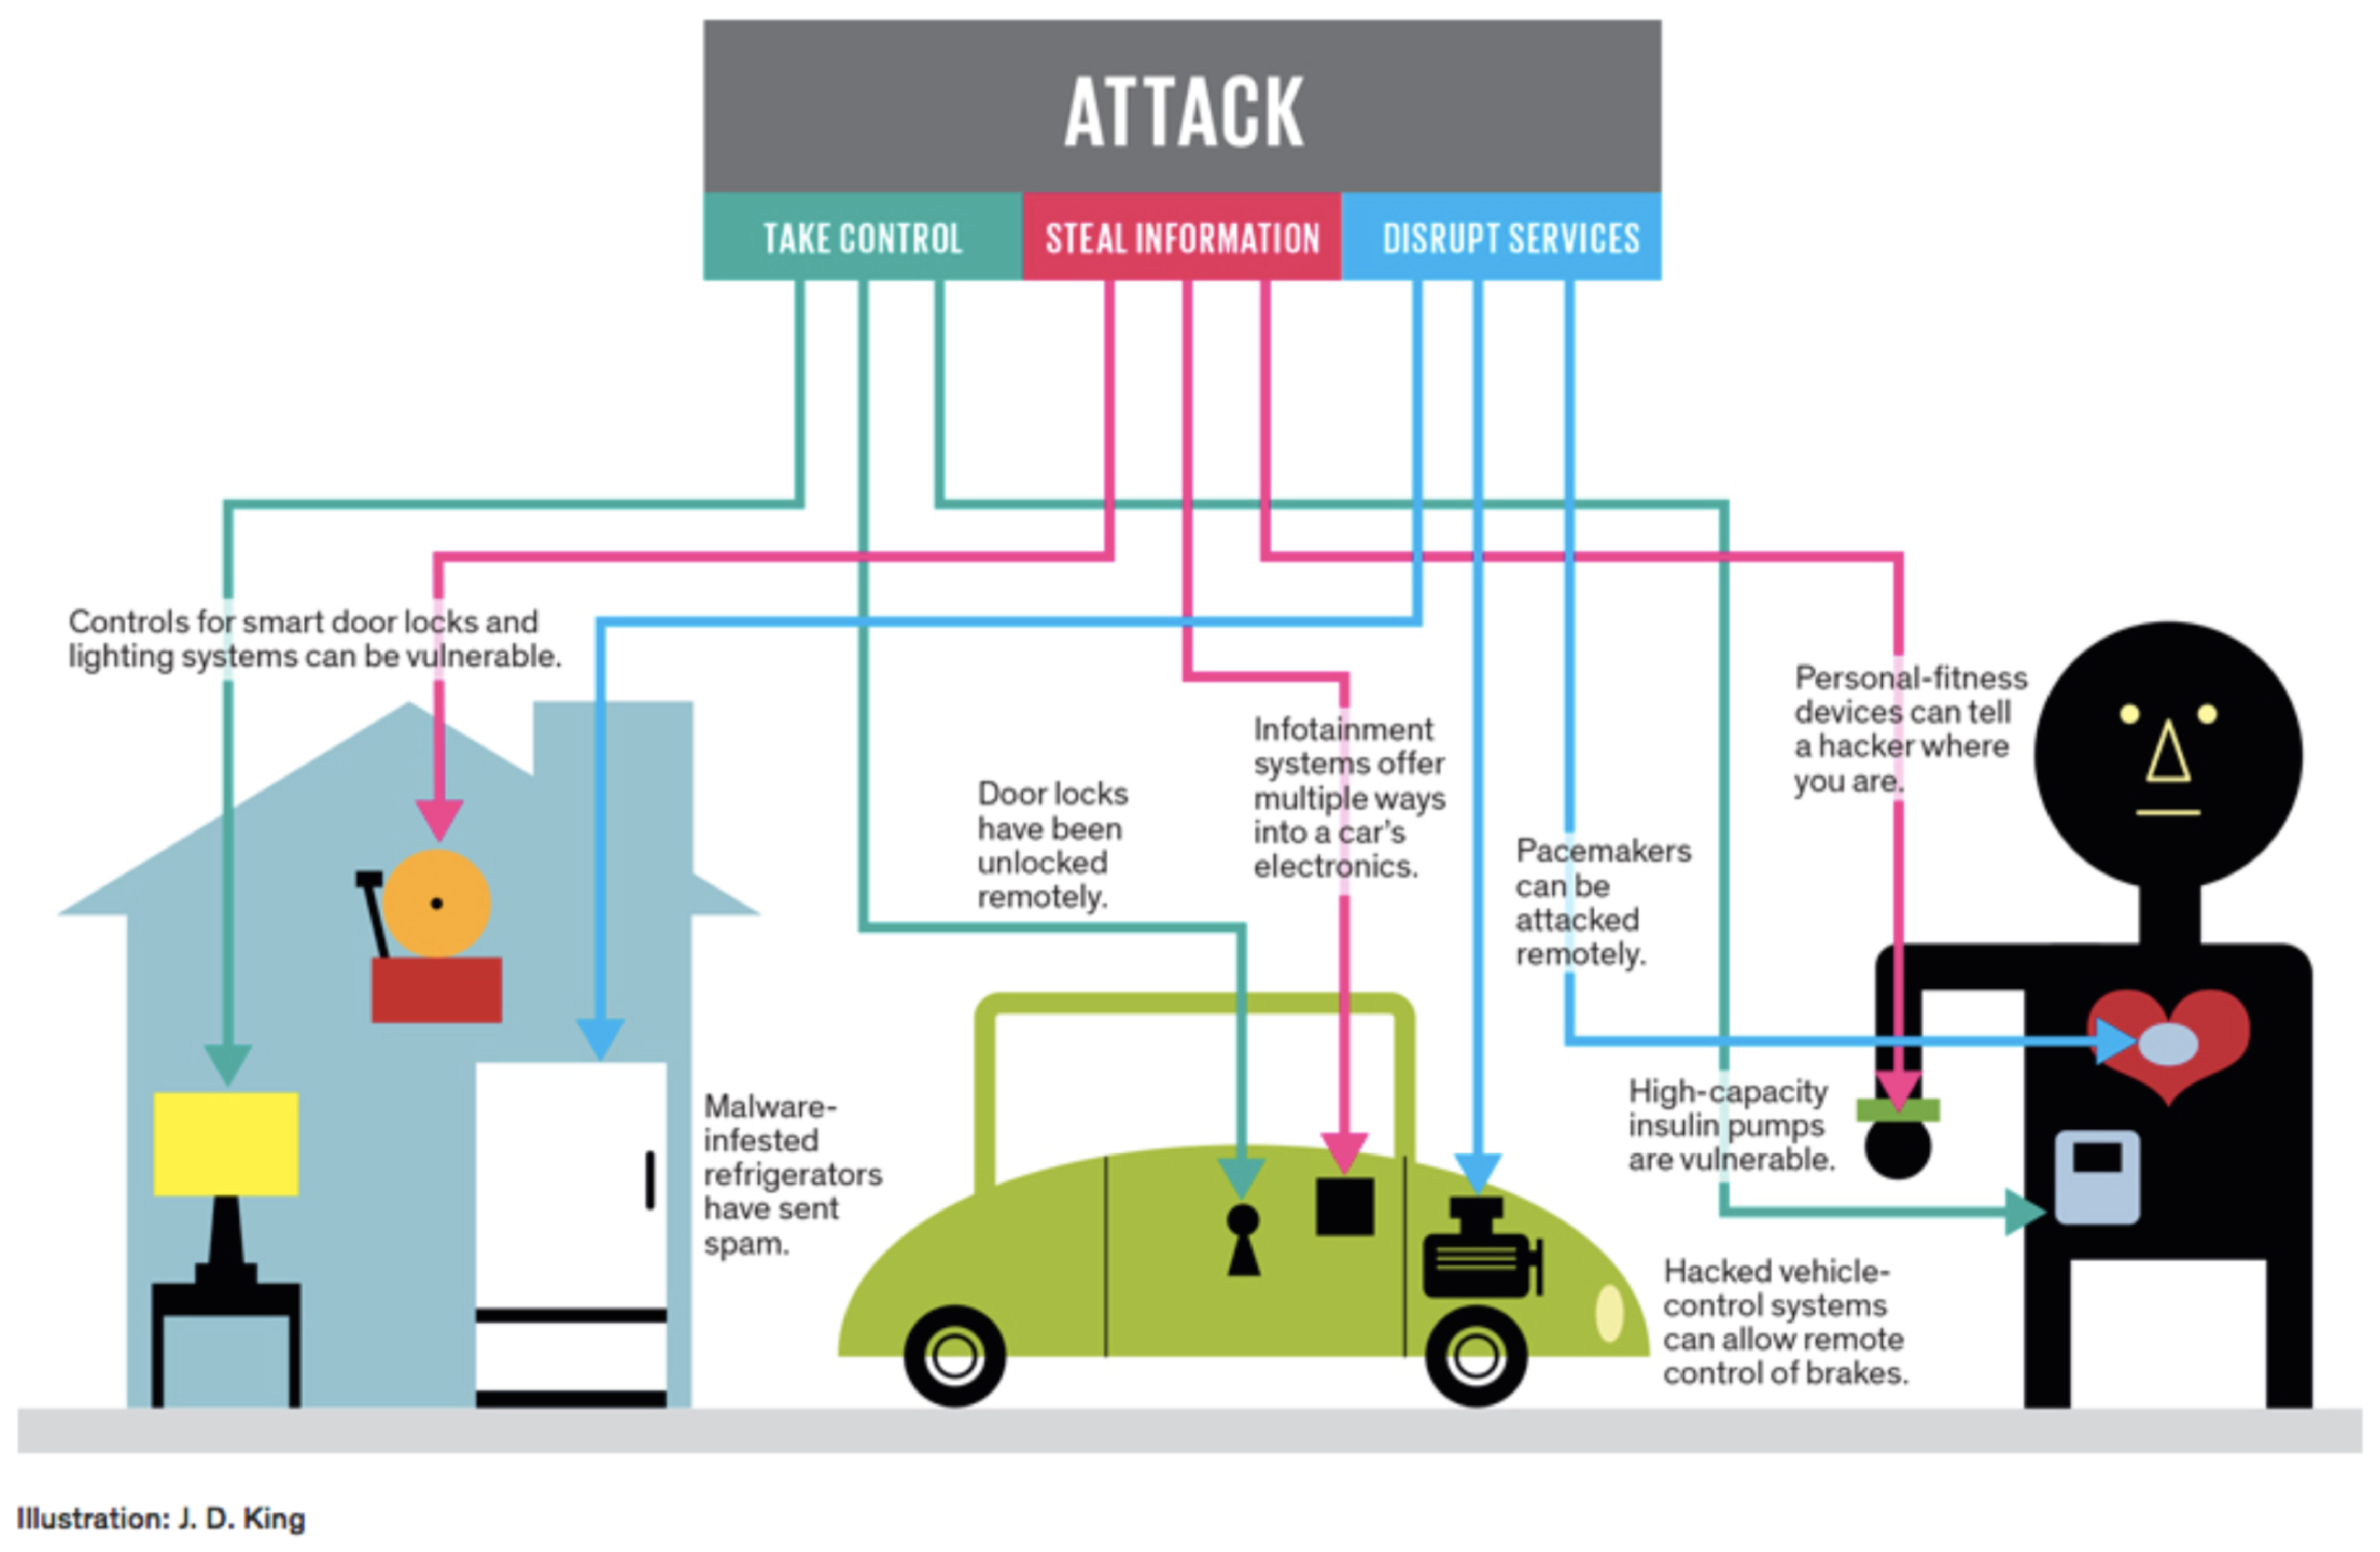
\includegraphics[height=4cm]{attack.eps}
    \end{column}
  \end{columns}
\end{frame}


% --------
% Slide 7
% --------
\begin{frame}
  \frametitle{\centerline{Smartcity}}
  \begin{block}{}
    Inteligentné mesto je vízia miest založená na integrácii informačných a komunikačných technológií
    (IKT) a internetu vecí (IoT) ktorá umožní bezpečným spôsobom spravovať majetok, infraštruktúru a zdroje v mestách.
  \end{block}
  \begin{center}
    \includegraphics[height=4cm]{smart_city.eps}
  \end{center}
\end{frame}


% --------
% Slide 8
% --------
\begin{frame}
  \frametitle{\centerline{Zdroje}}
  \begin{itemize}
    \item IoT – Internet Of Things \\
      {\scriptsize \url{https://www.meccanismocomplesso.org/en/iot-internet-of-things/}}
    \item What is the internet of things (and why does it matter)? \\
      {\scriptsize \url{http://www.businessit.cz/cz/internet-veci-v-praktickych-prikladech.php}}
    \item The Internet of Things Is Far Bigger Than Anyone Realizes \\
      {\scriptsize \url{https://www.wired.com/insights/2014/11/the-internet-of-things-bigger/}}
  \end{itemize}
\end{frame}

\begin{frame}
  \begin{center}
    \textbf{Ďakujem za pozornosť !}
  \end{center}
\end{frame}

\end{document}
